\documentclass[12pt]{article}
\usepackage{amsmath}
\usepackage{emptypage}
\usepackage{blindtext}
\usepackage{titlesec}
\usepackage{float}
\usepackage[hidelinks]{hyperref}
\usepackage{graphicx}
\usepackage[italian]{babel}
\graphicspath{ {./images/} }
\author{}
\title{
    \huge 
        \textbf{Università degli Studi di Modena e Reggio Emilia}
    \large
        \par Dipartimento di Scienze Fisiche, Informatiche e Matematiche
        \par Corso di laurea in Informatica
    \vfil
        \huge \par \textbf{Engim report service}
    \vfil
    \normalsize
    \begin{tabular}{lp{0.4\textwidth}l}
      Relatore: & & Candidato: \\
      Prof. Claudia Canali & &  Dumitru Frunza \\
      \end{tabular}
}
\date{Anno academico 2021/2022}
\linespread{1.5}



\begin{document}
\maketitle
\thispagestyle{empty}
\newpage 
\thispagestyle{empty}
\
\newpage
\pagenumbering{roman}
\addtocounter{page}{0}
\listoffigures
\newpage
\phantomsection
\tableofcontents
\addcontentsline{tesi}{Infrastruttura}{Infrastruttura}
\newpage
\pagenumbering{arabic}
\addtocounter{page}{0}


\phantomsection
\section*{Introduzione}
\addcontentsline{toc}{section}{Introduzione}
Un software gestionale è un sistema creato per aiutare un'azienda a organizzare 
e gestire il lavoro.
Engim offre la possibilità di monitorare le mansioni di un lavoratore e garantire 
la sua sicurezza tramite  ServizioGPS e TwiceTouch, i due prodotti di punta dell'azienda. 
In particolare, servizioGPS salva il percorso di una macchina lavoratrice e 
permette di calcolare il contributo dovuto. Ogni via attraversata viene salvata, 
ogni 5 secondi viene salvata una coordinata GPS.
\\ Nell'affrontare una grande quantità di dati, diventa importante
 disporre di un metodo affidabile e intuitivo per l'archiviazione degli stessi.
Un modo comune per salvare informazioni è tramite un file XLSX o PDF.
I file PDF sono semplici da usare, da interpretare e sono estremamente diffusi 
rendendoli perfetti per un cliente senza capacità tecniche. 
Un servizio simile può essere parte integrale del software in quanto effettivamente 
è un estensione dei servizi offerti. 
Questo è vero fin tanto che richiede minime risorse e tempo di calcolo.
\\ Cosa succede quando un servizio secondario, importante per i clienti ma non 
abbastanza da giustificare un grosso impegno da parte del server, pesa gravemente 
sul software? 
È il problema che sta affrontando Engim; il servizio di conversione da dati 
a PDf richiede troppe risorse per periodi prolungati rendendo difficile la user 
esperienze ma soprattutto sovraccaricando il server.
Intuitivamente si potrebbe migliorare la situazione attuale, andando a riscrivere 
il codice incriminato.
Questa soluzione però risolve solo il problema in termini di tempo e non di 
risorse, resta comunque un processo potenzialmente gravoso sulla macchina. 
Un altro possibile approccio sarebbe quello di scaricare delegare il calcolo.
\\ È possibile effettivamente astrarre il processo di conversione, portarlo su 
un servizio di terze parti migliorando performance e risparmiando risorse.

\thispagestyle{empty}
\newpage 
\thispagestyle{empty}
\
\newpage

\section{Engim Srl}
\subsection{L'azienda}
Engim è una società che si occupa di creare soluzioni tecnologiche in ambito 
ICT, telecomunicazioni, sistemi di gestione e mobilità. Da oltre 10 anni operano 
nel mercato della tracciabilità di flotte e attività e della 
sicurezza dei lavoratori in solitario.
\\ ServizioGPS è il noleggio di tracker gps per veicoli lavoratori. 
Una prevalente parte dei clienti sono comuni che, tramite i prodotti Engim, 
tracciano il percorso delle macchine spazzaneve e spargisale.
I tracker possono essere prodotti fisici oppure un app per smartphone. A loro 
volta i prodotti fisici si dividono in fissi e mobili. Il servizio include
anche un gestionale per poter visualizzare, modificare o archiviare i propri dati.
\\ Twicetouch è noleggio di dispositivi di sicurezza individuale.
Il prodotto tutela i lavoratori in solitario mandando una segnalazione in caso di
emergenza. Esistono due tipi di rilevazione: 
\begin{itemize}
  \item caduta: l'accelerometro del dispositivo rileva un urto pericoloso
  \item assenza di movimento: il lavoratore non si è mosso per un lasso prolungato di tempo, 
  quindi si presume che possa essere incosciente
\end{itemize}
Similmente a servizioGPS è possibile noleggiare un dispositivo fisico (badge) oppure
l'app per android. In entrambi i casi è possibile impostare i numeri in caso di 
emergenza, che riceveranno una chiamata e un messagio SMS.

\subsection{Infrastruttura}
Le tecnologie usate per servizioGPS sono le seguenti:
\begin{itemize}
  \item Ruby on rails full stack
  \item Mariadb e Redis come database
  \item Python come back end di supporto
  \item Java per il prodotti app 
\end{itemize}
\begin{figure}[H]
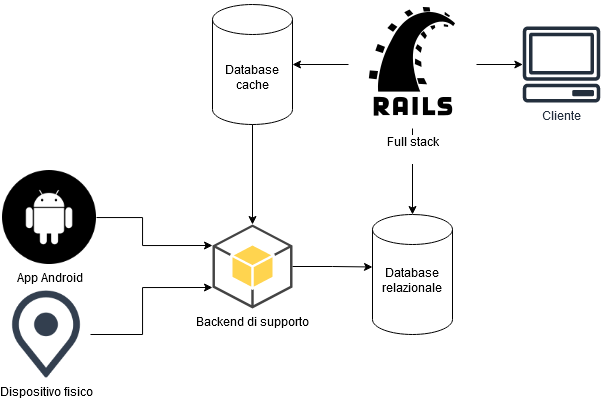
\includegraphics[scale = 0.6]{infrastructure.png}
\caption{Architettura}
\end{figure}
Ruby on Rails è usato per front-end e gran parte del backend di servizioGPS. 
Qualsiasi necessità front end side è responsabilità di Rails, questo è dove 
viene svolto la maggior parte della manutenzione siccome ha molte servizi diversi 
ed è a stretto contatto con il cliente.
Il Fetcher invece si dedica esclusivamente alla elaborazione di coordinate GPS. 
Questo non si trova sullo stesso server di Rails, bensi sul suo privato, molto 
più potente di quello di rails siccome è più vitale per il lavoro.
Le operazioni che fa sono poche quindi richiede poca manutenzione. 
Allo stesso scopo il servizio si appoggia su molteplici server, per quanto 
potente possa essere il backend potrebbe essere comunque eccessivo dover 
elaborare decine se non centinaia di migliaia di richieste contemporanee.
Uno di questi server è EC2.

% \subsection{Microservizi}
% Un servizio è un processo che: esegue specifiche operazioni autonomamente, 
% risponde a eventi oppure rimane in attesa di una richiesta. 
% Nel caso in cui queste operazioni vengano svolte continuamente, il servizio è 
% estremamente vantaggioso. Non è però necessario che il servizio sia sempre in 
% esecuzione se viene usato in maniera discontinua o per brevi periodi di tempo. 
% I microservizi coprono questo ruolo, hanno le stesse caratteristiche di un servizio
% ma eseguono solo su richiesta. 
% \\ L'ambiente di esecuzione è completamente gestito da AWS, l'unica requisito per 
% creare un microservizio è caricare il proprio codice. In questo caso viene 
% noleggiato il tempo di calcolo invece che una macchiana fisica o virtuale.
% L'ambiente viene creato al momento della richiesta, esegue il codice e cessa di 
% esistere. 
% Quando il microservizio non è attivo non ci sono costi.
% \\ È bene tenere in mente due importanti caratteristiche dei microservizi:
% \begin{itemize}
%   \item L'ambiente non ha spazio di archiviazione, qualora sia necessario 
%   salvare un file, bisogna caricarlo in un servizio di clound computing come S3
%   \item Le tecnologie devono essere compatibili con l'infrastruttura sottostante,
%   il che limita le nostre scelte
% \end{itemize}
% Avendo in mente queste considerazioni, un caso d'uso adatto ai microservizi 
% è un servizio API che viene usato in maniera occasionale oppure per brevi periodi 
% fissi.

\subsection{Sistema automatico di generazione di report}
Engim esegue una manutenzione annuale di database, che consiste nell'archiviazione
dei dati. Questi possono essere salvati dal cliente, nel caso fosse interessato 
o necessitato, sotto forma di pdf oppure xls.
\\ 
Le informazioni più importanti sono l'elenco e le specifiche di tutte le "attività". 
Un'attività contiente una serie di dati, tra cui: coordinate
gps, costi di lavoro, tempo di lavoro e altro.  
Al momento il servizio è implementato da Rails tramite una libreria di ruby. 
Il sistema attuale crea un istanza di chrome, l'istanza contiene un HTML
che si desidera convertire in pdf e infine avviene il parsing del documento.
\\ Questo ha una serie di gravi problemi:
\begin{itemize}
  \item La necessità di avviare un istanza di Chrome e il parsing di un HTML è
  estremamente costoso dal punto di vista delle risorse
  \item Il parsing di un HTML è anche estremamente costoso in termini di tempo,
  aggravato dalle lunghe query dovute alla grande mole di dati 
  \item Il  parsing tende a essere poco affidabile
\end{itemize}
La natura del nostro problema sembra molto adatta per il cloud computing.
L'operazione è ripetitiva, ben definita e usata per brevi periodi. Altri vantaggi 
importanti sono il risparmio di risorse del server, che evita di gravare sulle 
operazioni più critiche, e la possibilità di usare il progetto per qualsiasi 
altro prodotto Engim.

\section{Cloud computing}
\subsection{Introduzione}
Il cloud computing è una serie di servizi on-demand, generalmente di archiviazione 
e potenza di calcola, che non necessitano la gestione diretta da parte del utente. 
Il servizio viene erogato con un modello pay-as-you-go, ovvero si paga l'effettivo 
utilizzo invece che una quota fessa per un determinato periodo. 
Questo approccio aiuta a risparmiare soldi generalmente ma può portare a spese 
inaspettate, se il carico di lavoro dovesse subire un picco.
È un rischio che le grandi aziende sono felici di correre, infatti nel 2023 il 
mercato del cloud computing ha un valore di 706 miliardi. Si stima che entro il 
2025 il numero crescerà fino a 1.8 bilioni. 
\\ L'idea di condividere risorse non è nuova, bensì nasce nel 1960. Al tempo 
un ufficio aveva un mainframe con varie postazioni. Ogni macchina poteva fare 
una richiesta tramite un job e doveva aspettare l'esecuzione: remote job entry.
Nel 1990 le aziende di telecomunicazioni sono passate da connessioni 
point-to-point a virtual private network.
La performance non ha subito alcun miglioramento ma adesso era possibile 
decidere come impiegare le risorse. I clienti ricevevano banda in base 
alla loro richiesta, questo risultava in un grosso risparmio per l'azienda.
\\ Il pioniere del cloud computing come lo conosciamo oggi è stato Amazon che 
nel 2002 Amazon Web Services.

\subsection{AWS}
Amazon Web Services è una susidiaria di Amazon che offre servizi di cloud 
computing e APIs per individui, aziende e governi.
Un servizio molto popolare è l'autoscaling, ovvero un server capace di aumentare 
di potenza quando ha bisogno di più potenza senza ausiglio umano. 
Uno dei serivzi più importanti di amazon è Amazon Elastic Compute Clound (EC2), 
un cluster di computer usabili tramite REST API, CLI o AWS console. Questi 
computer simulano in tutto e per tutto un server tradizionale, ma non hanno 
un unità di memoria. 
È quindi necessario usare un servizio di storage, sia per i dati testuali 
quindi un database sia per i dati multimediali. 
\\ Amazon aurora se fosse necessario avere un servizio di database compatibile 
con mysql. 
\\ Amazon Dynamo DB, se service un database caching. 
\\ Amazon S3 per archiviazione di dati multimeddiali.
Ma è anche possibile anche dividere la logica in molteplici parti, tramite un 
architettura a microservizi

\subsection{Microservizi}
Un architettura a microservizi indica una serie di componenti separati che 
possono essere sviluppati e rilasciati in maniere indipendente. 
I prodotti amazon che permetto queste semplicita sono amazon sns, per i notifiche
amazons sqs per i messaggi e amazon lambda per il codice. 
Particolarmente interessante è labmda, che è una funzione senza casa.
È un codice che non è attivo per la maggior parte del tempo, quando riceve una 
richiesta viene creato il suo ambiente e risponde al servizio. 
Quindi permette di portare fuori dal server piccoli pezzi di logica specifica, 
e eseguirli su un ambiente pulito e veloce. 
È possibile quindi fare un implementazione veloce, modulare e evitare di 
sovvracaricare il prodotto principale. 
Rispetto a un modello tradizionale a servizi permette di risparmiare molta 
potenza di calcolo e scala molto facilmente. 
Nel caso però in cui si parla di processi naturalmente non è molto adatto.

\section{Requisiti del progetto}
\subsection{Descrizione}
Il progetto è una funzione lambda su AWS, ovvero un microservizio. La funzione 
viene chiamata in maniera diretta tramite una libreria di ruby.
Questa richiede le credenziali IAM per effettuare l'accesso alla lambda e prende 
in input un JSON. Al suo interno abbiamo un token di autenticazione e il dominio 
di provenienza che vengono controllati dalla lambda. 
\\ I contenuti invece sono divisi in sezioni per permettere dinamicità di stampa, 
qualora uno dei blocchi fosse assente, semplicemente non verrà stampato. 
\\ Nel caso in cui la stampa sia avvenuta correttamente la funzione ritorna 
"200 OK"
e il nome del file su S3. Se l'input della chiamata risulta errato, la funzione ritorna 
"400 BAD REQUEST"
e un messaggio che descrive l'errore. Infine se avviene un errore di connessione 
al bucket S3, la funzione ritornerà un errore "500 INTERNAL ERROR".    
\\ Il progetto deve permettere l'implementazione di stampe diverse da quelle di servizioGPS
e di altri file di output come KML e XLSX. 

\begin{figure}[H]
\includegraphics[width =\textwidth]{realUseCases.png}
\caption{Casi d'uso}
\end{figure}



\subsection{Sicurezza}
L'autenticazione avviene a livello di codice, sia sul server che sul microservizio.
\\ La libreria "aws-sdk-lambda" permette di stabilire una connessione diretta con la 
lambda. È sufficiente fornire: nome della funzione, regione, credenziali e payload. 
Le credenziali sono salvati dentro un file crittografato yaml. 
Un ulteriore livello di sicurezza è integrato nella funzione sotto forma 
di token e whitelist. 
\\ Questi valori sono salvati nel ambiente di AWS, per evitare di averli 
scritti in chiaro nel codice. Il token è un lungo carattere alfanumerico.
\\ La whitelist contiene tutti i domini di Engim, questi vengono caricati in 
una lista e confrontati con il mittente. 
Nel caso in cui 
l'operazione sia andato a buon fine, ritornerà un JSON in risposta.
\\ Qualsiasi chiamata da dominio esterni oppure senza token verrà tratta come 
"400 BAD REQUEST". 

\subsection{Correttezza dei dati}
Esistono 3 blocchi principali: "header", "body", "table".
Fin tanto che almeno uno dei 3 è presente, la stampa risulta valida.
Facoltativamente è possibile includere il blocco "media", che contiene 
eventuali immagini in "base64". 
\\ Il header può contenere fino a 2 loghi, però deve necessariamente avere 
un titolo e una intestazione. 
Uno dei due loghi è sempre quello aziendale, mentre l'altro può essere una copia 
del precedente oppure appartenere al cliente.
L'intestazione racchiude: dominio di provenienza, nome utente e data di oggi.
\\ Il body può avere un numero arbitrario di blocchi. Ogni blocco è racchiuso 
in un rettangolo e anche esso ha una serie di titoli con i loro dati. 
È valida l'assenza di un dato, ma invalida l'assenza di un titolo. 
\\ Il table è composto da una serie di titoli e una serie di righe. Non c'è limite 
al numero di righe che può contenere.
Anche in questo caso non può mancare un titolo ma un dato può essere vuoto. 
\\ Tra i tipo di dato, di una tabella, 
è possibile avere un immagine che viene spedita in 
base64, se è assente non verrà scritto nulla. Onde evitare la duplicazione 
eccessiva di immagini, siccome una tabella potenzialmente contiene un numero 
illimitato di dati, le immagini sono salvate nel blocco media in singola coppia. 
\\ Il programma presume che i dati siano corretti, controlla solo la loro presenza.
La funzione anche presume che ogni dato sia una stringa, questo evita conversioni 
e permette di stampare qualsiasi dato a prescindere dalla provenienza.

\subsection{Problemi interni del server}
Durante l'esecuzione vengono effettuate delle connessioni dirette tra i servizi. 
In un primo momento Rails si collega con la lambda, questa connessione potrebbe 
essere soggetta a timeout. 
\\ Lambda a sua volta crea un canale con il bucket, per poter 
effettuare il caricamento del file, qualsiasi tipo di errore viene catturato da javascript.
Nel caso in cui il file venga salvato correttamente,
la lambda restituisce la chiave del file, ovvero il suo nome. 
\\ Infine Rails si collega al bucket e cerca il link per aprire o scaricare il file 
direttamente dal bucket.
Questa connessione può sembrare superflua, ma aggiunge 
un livello di sicurezza ulteriore senza aumenti degni di nota sul costo temporale. 


\subsection{Presupposti e dipendenze}
Siccome AWS mette a disposizione l'infrastruttura c'è una scelta limitata dei 
linguaggi di programmazione.
Nella lista sono presenti i più popolari al momento,
in particolare sono stati presi sotto esame python, ruby e javascript.
\\ Ruby ha numerose librerie che permettono la scrittura dei PDF che purtroppo
prevedono il parsing di un HTML.
Questa operazione è molto vantaggiosa per lo sviluppo ma non particolarmente 
per l'efficienza.
Ogni conversione richiede un istanza di chrome da cui convertire il file,
creando una serie di processi non necessari.  
\\ Python offre molteplici librerie, ognuna con diverse funzionalità. Non è 
sufficiente usarne sol una per le operazione desiderate e inoltre 
molte di queste librerie non sono mantenute in maniera costante
\\ Javascript invece ha "pdfkit", una libreria che permette la creazione e manipolazione 
di un PDF senza intermezzi. È molto popolare, open source con una comunità 
attiva, oltre ad avere una documentazione breve e chiara.
\\ La stampa ha una forma regolare, divisa per righe e colonne. Se i dati sono 
disposti in maniera più arbitraria è necessaria un implementazione diversa. 
Non è richiesto la stampa in altri formati di file, ma è necessario lasciare 
la libertà di aggiungere diversi formati in futuro.

\subsection{Features}
La lambda ha un unica funzionalità, stampa e salvataggio della stampa.
\begin{figure}[H]
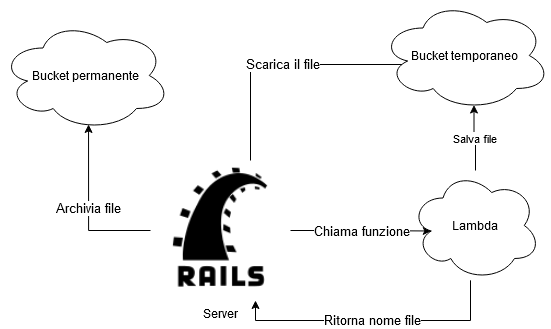
\includegraphics[scale = 0.6]{useCases.png}
\caption{Schema logico}
\end{figure}
Ogni stampa deve seguire seguire lo schema a blocchi definito, non è possibile 
ad esempio affiancare un immagine in una tabella. 
Qualsiasi implementazione che non segua lo standard va aggiunta alla funzione.
\\ È possibile stampare immagini. Queste devono essere prese in input siccome non 
esiste una memoria permanente per la funzione.
\\ Ogni file viene salvato su lambda, con il nome che è data e ora di oggi. 
Lambda automaticamente crea cartelle divise per mese e per giorni. 
Una volta che il file è stato salvato, rails può pescare il file e mostrarlo 
o lasciare il download per l'utente.
\\ Il bucket temporaneo viene svuotato periodicamente, se un dato serve per il 
cliente verrà salvato sul bucket permanente. 
Se invece il cliente non se lo tiene per conto suo verrà cancellato nel tempo.
\\ Il motivo per la divisione dei bucket è per dividere la logica, io non voglio 
che la mia lamda si occupi del organizzazione dei file, come non voglio 
che rails metta le mani nel bucket di lambda, quindi si salva tutto nel suo.



\section{Implementazione}
\subsection{Flusso di lavoro}
È stato deciso di lavorare con continua integrazione. 
\\ In prima battuta creare una funzione in grado di generare un PDF e salvarlo 
su S3. Testare ogni aspetto della funzione ed effettuare il deploy su AWS. 
\\ Successivamente integrare la funzionalità in rails, eliminando la vecchia 
funzione. Assicurarsi che la stampa esegue correttamente ed in tempi ragionevoli.

\subsection{Creazione di un file e salvataggio su S3}
È possibile interagire con un bucket S3 tramite due modi: connessione con link 
creato da un utente autorizzato oppure connessione IAM. In questo particolare 
caso è necessario stabile una connessione diretta tramite IAM. Una volta stabilita 
è possibile accedere a una serie di metodi tra cui "upload()". Al termine del 
caricamento il bucket ritorna un dizionario con una serie di informazioni, la 
più importante è la chiave, che è il nome del file su S3. Nota importante, 
non usare "key" perché è un valore vecchio per retrocompatibilità, bensi "Key". 

\subsection{Generazione di un PDF da un JSON}
La libreria permette scrittura sul file, disegno elementare e manipolazione di 
font, posizione e colore.
Inizialmente appariva conveniente un approccio funzionale, ma vedendo il modo 
particolare in cui viene esportato un file in "Nodejs" e la complessità sempre 
maggiore dei documenti, è stato deciso di creare una classe: PdfDocument. 
\\
Il costruttore va a definire la grandezza del documento in base al blocco più 
largo del file.
Questa definisce la larghezza del documento e l'altezza viene calcolata di
conseguenza (1.41 volte più grande, come un foglio A4).
Il formato default è A4, per evitare stampe troppo piccole.
Mantenendo queste proporzioni la visualizzazione e la stampa risultano molto 
semplici.
Una volta definito il documento la classe chiama il metodo "writeData()".
Questo controlla la presenza dei dati e richiama altri metodi di scrittura 
se necessario.
I metodi di scrittura controllano che non manchino dati vitali e se così non fosse 
scrivono sul documento. 
È possibile richiedere il documento tramite "getDocument()". 
\\ Il file è uno stream di dati e può essere spedito direttamente su S3. 

\begin{figure}[H]
\includegraphics[]{uml.png}
\centering
\caption{Casi d'uso}
\end{figure}

\subsection{Test automatizzati}
Si è deciso di effettuare del "unit testing" tramite la libreria mocha.
Ogni singolo modulo è testato singolarmente con dati corretti ed errati. 
Ogni input è generato casualmente grazie a "faker-js". 
Infine le connessioni con AWS sono simulate tramite "aws-sdk-dev". 

\subsection{Ruby on Rails}
Il metodo di stampa corrente ritorna una pagina HTML e richiede la stampa oppure 
scarica la conversione di quella pagina. Innanzitutto è necessario cambiare il 
ritorno da HTML a PDF e in seguito passare un valore alla chiamata per distinguere 
la visualizzazione dallo scaricamento del file. 
La prossima fase è caricare tutti i dati in un hash e trasformarlo in un JSON. 
Ogni stampa ha disposizioni simili ma una conversione dei dati diversa, è quindi 
necessario creare due distinte funzioni: una per le attività e una per la singola 
attività
\\ Una volta definito il JSON si può stabile una connessione diretta con la lambda e 
chiamare il metodo interessato.
Al termine della chiamata il metodo ritornerà il nome del file e stabiliamo un
ulteriore connessione, stavolta col bucket, per visualizzare o scaricare il file.
Il ritorno di questa richiesta è un JSON che
contiene una serie di link tra cui il url di download e il url di visualizzazione.
Il motivo per cui questo non viene ritornato direttamente dalla lambda è per avere 
un livello di sicurezza extra. 

\section{Applicazione e performance}
\subsection{Risultati}
Non è stato necessario cambiare nessuna parte dell'interfaccia grafica.
Sul nav della sinistra sono presenti una serie di funzioni di servizioGPS, 
l'unica di nostro interesse è Activities, e una serie di dati extra. 
Il primo grosso blocco è un classico blocco di ricerca che permette 
di trovare attività specifiche.
È possibile stampare una lista di attività cliccando sulla stampante oppure una 
scaricarle cliccando sul immagine alla sua destra, infine è possibile spedirle 
per mail traite la lettera. 
Il blocco sottostante è un riassunto delle attività, è compreso nella stampa. 
Infine segue una tablle con tutti i dati importanti: id, stato, 
prima posizione, ultima posizione, tipo, dispositivo, utente, 
azienda e servizio in totale. 
\begin{figure}[H]
\includegraphics[width =\textwidth]{lista_attività.jpg}
\caption{Lista di attività}
\end{figure}
Di seguito è possibile vedere un esempio di stampa di attività. 
In alto è possibile trovare il server di provenienza, con tanto di data e 
azienda.
A destra è scritta la versione del software della lambda. 
Il header è il blocco con il titolo e il logo di serviziogps.
Il body è il blocco che riassume il blocco visto nell'immagine precendente. 
Il table è l'elenco di tutte le attività, che è identico a quello sul server, 
esclusa l'ultima posizione.
In questo caso sono presenti 6 attività, ma possono essere fino a 20 mila. 
\begin{figure}[H]
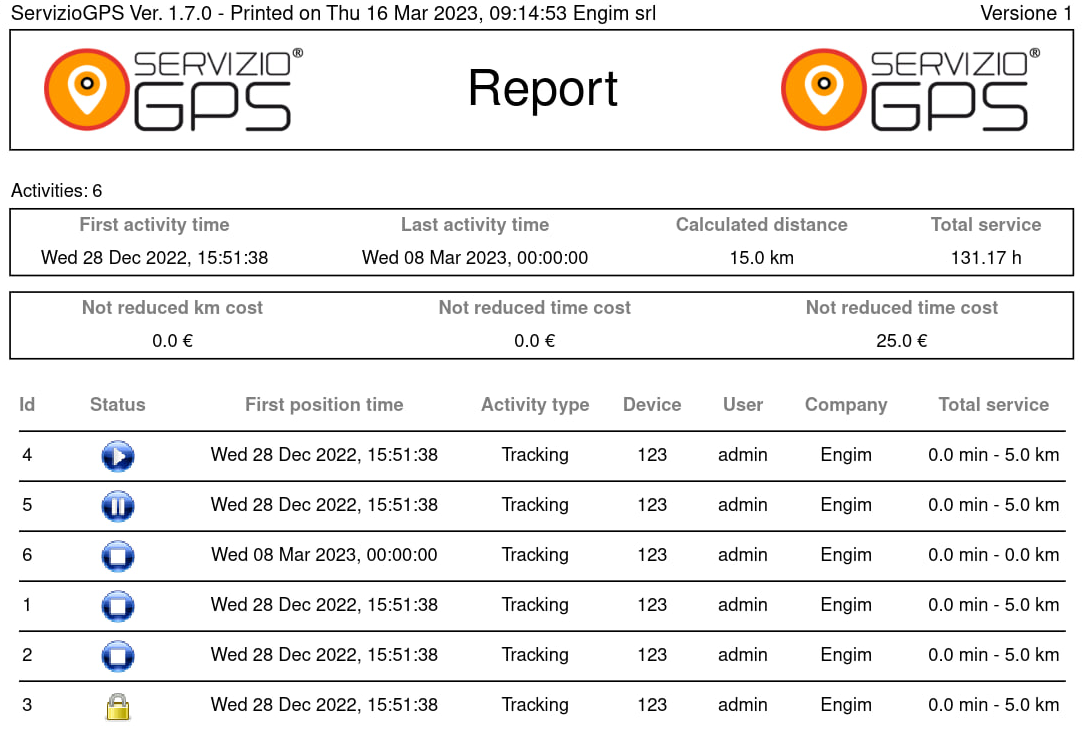
\includegraphics[width =\textwidth]{report.png}
\caption{Stampa del elenco attività}
\end{figure}

Alternativamente è possibile stampare i dettagli di un unica attività. 
In questa pagina è possibile vedere nel dettaglio il percorso fatto 
dal dispositivo, i punti gps e la rapresentazione sulla cartina. 
\begin{figure}[H]
\includegraphics[width =\textwidth]{singola_attività.png}
\caption{Attività visualizzazione}
\end{figure}
Esempio di stampa di un attività 
\begin{figure}[H]
\includegraphics[width =\textwidth]{report_attività.png}
\caption{Stampa di una singola attività}
\end{figure}
In questo caso è presente solo una via ma è possibile averne potenzialmente 
fino a 20 mila. Ogni singolo blocco fa parte del blocco in alto.  
Oltre al logo di serviziogps è presente anche il logo del comune o azienda 
se è presente. 

\subsection{Performance}
Sono stati fatti test di performance sul elenco delle attività siccome è la 
stampa più impegnativa, perché contiene molte immagini.  
\begin{figure}[H]
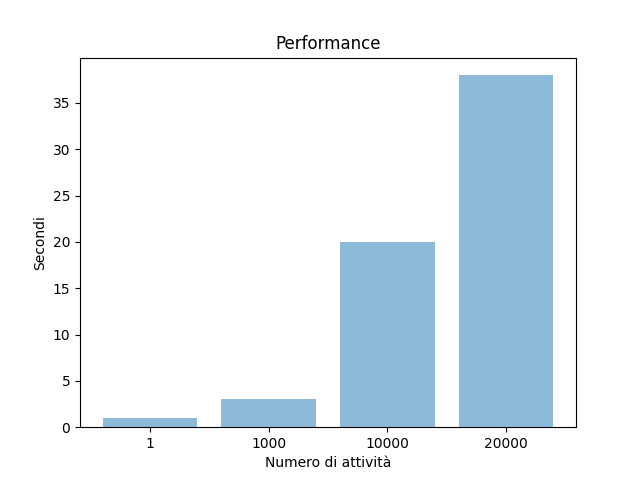
\includegraphics[width =\textwidth]{performance.png}
\caption{Performance}
\end{figure}
Al aumentare delle attività aumenta in maniera quasi lineare il tempo. Questo 
è dovuto al numero alto di cicli di scrittura.
Oltre venti mila attività non è possibile effettuare una stampa perché 
raggiungiamo il limite del buffer di AWS. Se fosse necessario aumentare 
la performance sarebbe sufficiente trasformare le immagini in icone vettoriali.
\\ Altre possibile ottimizzazione potrebbero essere: definire a priori le 
misure del foglio e salvarle come costanti oppure modificare il JSON per 
semplificare la struttura dati. 
Tuttavia non è necessario perché sono tempi ragionevoli.
È più importante notare che il server usi risorse minime, in quanto deve 
solo aspettare il ritorno della chiamata https. Questo era il fulcro del progetto, 
permettere una migliore e più sicura navigazione alleggerendo il lavoro compiuto 
dal software.
\\ L'implementazione precedente aveva una performance ottima per un numero ridotto 
di informazioni, 
siccome non era legata a dei tempi fissi di connessioni. Allo stesso tempo al 
crescere delle attività aumentava esponenzialmente il tempo e rendeva alto il 
rischio di crash.


\thispagestyle{empty}
\newpage 

\phantomsection
\section*{Conclusione}
\addcontentsline{toc}{section}{Conclusione}
I microservizi offrono un nuovo paradigma di programmazione, uno dove è possibile 
astrarre logica dal proprio software e eseguirla solo qual'ora fosse necessario. 
È possibile condividere questa logica su diversi piattaforme, e permette una 
scalabilità semplice e veloce.
Naturalmente non è adatto a ogni situazione situazione. Una serie di operazioni 
numerose o estremamente lunghe richiedono un servizio. 
Nel caso studiato invece una lambda è estremamente vantaggiosa.
\\ In primo luogo risolve il problema del sovraccarico del server. Migliorare la 
logica e gli algoritmi sarebbe stato corretto ma non avrebbe alleggerito il carico 
di lavoro. L'esportazione del servizio invece permette di mantenere massima 
performance del sito siccome i calcoli vengono fatti altrove.
\\ Il costo temporale non ha subito migliorie nei casi più semplici, ma cresce 
in maniera lineare al aumentare della mole di lavoro. Questo è molto più importante, 
perché ci garantisce usabilità anche nei casi più estremi, visto che non è 
poco comune avere una grossa mole di dati. 
\\ Il progetto si era concentrato sulle stampe più impegnative, siccome erano 
quelle responsabile del impatto negativo sul software e siccome sono le più 
comuni. Non sono però le uniche stampe presenti sul server. Esistono varie 
informazioni da stampare che sono meno vitali e meno usate.
È però corretto avere una logica unica per tutte e portarla su lambda. 
\\ Inoltre non è possibile scaricare solo in formato PDF, bensì anche in XLSX e 
KML. È possibile introdurre queste tipologie in futuro, naturalmente ognuno 
dovrà avere una sua implementazione personale. 
Cosicché ogni operazione di stampa è estratta dal server ed è in un 
unico progetto centrale.
Questo permetterebbe al Rails di concentrarsi esclusivamente sul esposizione
dei dati ai clienti.

\thispagestyle{empty}
\newpage 

\phantomsection
\section*{Bibliografia}
\addcontentsline{toc}{section}{Bibliografia}

\begin{thebibliography}{9}
  \bibitem{link}
  AWS documentazione. 
  \url{https://docs.aws.amazon.com/lambda/index.html}

  \bibitem{link}
  Ruby documentazione.
  \url{https://ruby-doc.org/}

  \bibitem{link}
  Rails documentazione.
  \url{https://api.rubyonrails.org/}

  \bibitem{link}
  Nodejs documentazione.
  \url{https://nodejs.org/it/docs}

  \bibitem{link}
  Mozilla documentazione.
  \url{https://developer.mozilla.org/en-US/}

  \bibitem{link}
  Pdf-kit documentazione.
  \url{https://pdfkit.org/}

  \bibitem{link}
  Microservizi wiki.
  \url{https://en.wikipedia.org/wiki/Microservices}

  \bibitem{link}
  Cloud computing wiki.
  \url{https://en.wikipedia.org/wiki/Cloud_computing}


  \bibitem{link}
  Amazon Web Service wiki.
  \url{https://en.wikipedia.org/wiki/Amazon_Web_Services}

  \bibitem{link}
  Remote job entry wiki.
  \url{https://en.wikipedia.org/wiki/Remote_job_entry}

  \bibitem{link}
  Amazon aurora.
  \url{https://aws.amazon.com/it/rds/aurora/?nc2=h_ql_prod_fs_aa}

  \bibitem{link}
  Amazon DynamoDB
  \url{https://aws.amazon.com/it/dynamodb/?nc2=h_ql_prod_fs_ddb}

  \bibitem{link}
  Amazon S3.
  \url{https://aws.amazon.com/it/s3o /?nc2=h_ql_prod_fs_s3}


  \bibitem{link}
  Amazon SNS.
  \url{https://aws.amazon.com/it/sns/?nc2=h_ql_prod_ap_sns}

  \bibitem{link}
  Amazon SQS.
  \url{https://aws.amazon.com/it/sqs/?nc2=h_ql_prod_ap_sqs}

  \bibitem{link}
  Amazon Lambda.
  \url{https://aws.amazon.com/it/lambda/?nc2=h_ql_prod_cp_lbd}

\end{thebibliography}


\end{document}